
\documentclass{article} % For LaTeX2e
\usepackage{iclr2026_conference,times}


\usepackage{booktabs}
\usepackage{xcolor}
\usepackage{xspace}
\usepackage{tikz}
\usetikzlibrary{fit,backgrounds,arrows.meta}
\pgfdeclarelayer{background}
\pgfsetlayers{background,main}
\usetikzlibrary{positioning,calc}
\usepackage{booktabs}
\usepackage{graphicx}
\usepackage{dsfont}
% \usepackage[ruled,vlined]{algorithm2e}
\usepackage{makecell}
\usepackage{pgfplots}\pgfplotsset{compat=1.17}
\usepackage{multirow}
% \usepackage{hyperref}
\usepackage{url}



\usepackage[margin=1in]{geometry}
\usepackage{amsmath,amssymb,amsthm,bm,mathtools}
\usepackage{booktabs}
\usepackage{algorithm}
\usepackage{algpseudocode}
\usepackage{tikz}
\usetikzlibrary{positioning,arrows.meta,fit,calc}
\usepackage[colorlinks=true,linkcolor=blue,citecolor=blue,urlcolor=blue]{hyperref}


\newtheorem{definition}{Definition}
\newtheorem{remark}{Remark}

% Rename the method here.
\newcommand{\method}{\textsc{Method}}
\newcommand{\dpuct}{\textsc{D-PUCT}}
\newcommand{\sdpo}{\textsc{SDPO}}
\newcommand{\grpo}{\textsc{GRPO}}
\newcommand{\sg}{\operatorname{sg}}
\newcommand{\Dset}{\mathcal{D}}
\newcommand{\Mem}{\mathcal{M}}
\newcommand{\Tree}[1]{\mathcal{T}(#1)}
\newcommand{\Ch}[1]{\mathcal{C}(#1)}
\newcommand{\Act}[1]{\mathcal{A}(#1)}
\newcommand{\vchild}{\hat{s}}
\newcommand{\sota}{\mathrm{sota}}


\newtheorem{proposition}{Proposition}
\newtheorem{corollary}{Corollary}
\newcommand{\norm}[1]{\left\lVert #1\right\rVert}
\newcommand{\inner}[2]{\left\langle #1,#2\right\rangle}
\newcommand{\op}{\mathrm{op}}
\newcommand{\adv}{\mathrm{adv}}
\newcommand{\base}{\mathrm{base}}
\allowdisplaybreaks


\newcommand{\tba}{\textcolor{red}{??}\xspace}   % "to be added" placeholder
\newcommand{\ASR}{\mathrm{ASR}}



\definecolor{envgray}{HTML}{ECEFF4}
\definecolor{blockblue}{HTML}{7189B0}
\definecolor{llmteal}{HTML}{5A8474}
\definecolor{rldark}{HTML}{7B1F1F}
\definecolor{hdrgray}{HTML}{B5B5B5}
\definecolor{rowgray}{HTML}{EDEDED}
\definecolor{diffga}{HTML}{C8E4C5}
\definecolor{diffgb}{HTML}{DFF0DD}
\definecolor{diffba}{HTML}{D6E8F7}
\definecolor{diffbb}{HTML}{BBD7F0}
\definecolor{cardgray}{HTML}{DEDEDE}
\definecolor{prgray}{HTML}{C9C9C9}



\usepackage{hyperref}
\usepackage[all]{hypcap}


\title{Evolve}

\author{Antiquus S.~Hippocampus, Natalia Cerebro \& Amelie P. Amygdale \thanks{ Use footnote for providing further information
about author (webpage, alternative address)---\emph{not} for acknowledging
funding agencies.  Funding acknowledgements go at the end of the paper.} \\
Department of Computer Science\\
Cranberry-Lemon University\\
Pittsburgh, PA 15213, USA \\
\texttt{\{hippo,brain,jen\}@cs.cranberry-lemon.edu} \\
\And
Ji Q. Ren \& Yevgeny LeNet \\
Department of Computational Neuroscience \\
University of the Witwatersrand \\
Joburg, South Africa \\
\texttt{\{robot,net\}@wits.ac.za} \\
\AND
Coauthor \\
Affiliation \\
Address \\
\texttt{email}
}
\definecolor{envgray}{HTML}{ECEFF4}
\definecolor{blockblue}{HTML}{7189B0}
\definecolor{pillblue}{HTML}{9FB4D4}
\definecolor{llmteal}{HTML}{5A8474}
\definecolor{rldark}{HTML}{7B1F1F}
\definecolor{hdrgray}{HTML}{B5B5B5}
\definecolor{rowgray}{HTML}{EDEDED}
\definecolor{diffga}{HTML}{C8E4C5}
\definecolor{diffgb}{HTML}{DFF0DD}
\definecolor{diffba}{HTML}{D6E8F7}
\definecolor{diffbb}{HTML}{BBD7F0}
\definecolor{cardgray}{HTML}{DEDEDE}
\definecolor{prgray}{HTML}{C9C9C9}

\newcommand{\fix}{\marginpar{FIX}}
\newcommand{\new}{\marginpar{NEW}}

%\iclrfinalcopy % Uncomment for camera-ready version, but NOT for submission.

% Example citation to populate bibliography

\begin{document}



\maketitle

\begin{abstract}
\cite{Bengio+chapter2007}
\end{abstract}




\section{Problem Setup and Notations}
\label{sec_setup}

Scientific discovery often depends on finding one exceptional solution among many unsuccessful attempts. This objective differs from settings in which an agent is evaluated by the average quality of its outputs. We therefore model agentic scientific discovery as a search whose success is determined by the best valid candidate produced during the search.
A problem description $d$ specifies the candidate space, the validity requirements, and the evaluation procedure. Examples include discovering an efficient kernel implementation, constructing a numerical method, or identifying an object that satisfies a collection of scientific constraints. The agent interacts with this problem by repeatedly proposing and evaluating candidate solutions.

\begin{definition}[Agentic Discovery]
\label{def:sci}
Let $s_t$ denote the candidate available at search step $t$. The initial state $s_0$ may be empty or may contain a provided baseline solution. Conditioned on the problem description, the current candidate, and the accumulated search context, the language model generates an action $a_t$ containing a proposed modification together with any executable code required to realize it. A problem-dependent transition function constructs the next candidate according to
$s_{t+1} = T_d(s_t, a_t).$
An evaluator assigns each candidate a scalar reward $R_d(s)$ and textual feedback $F_d(s)$. The reward measures candidate quality under the task-specific evaluation procedure. Candidates that violate validity requirements receive zero reward. Let $r_{\sota}$ denote the reward of the strongest previously known valid solution. A discovery is made when the search produces a candidate $s$ satisfying
\begin{equation}
R_d(s) > r_{\sota}.
\end{equation}
\end{definition}


The objective in Def.~\ref{def:sci} places no direct requirement on the average reward of generated candidates. A search procedure may therefore explore uncertain or initially unpromising directions when doing so increases the probability of producing one substantially better solution.
The generation process induces a rooted search tree. Each node corresponds to an evaluated candidate, and each edge records the action used to derive a child candidate from its parent. The root is the initial state $s_0$. We also maintain the flat archive $\Dset_B$, which contains every evaluated node regardless of its location in the tree. The tree preserves local search trajectories, while the archive provides a global record of the solutions and evidence collected throughout the search.

For a node $s$, let $\Tree{s}$ denote the subtree rooted at $s$, including $s$ itself. Let
$m_s = \lvert \Tree{s} \rvert$
denote the number of evaluated candidates in this subtree. We assign each node its observed candidate quality
$Q(s) = R_d(s).$
When the subtree contains $m$ evaluated nodes, we summarize its demonstrated discovery value using
\begin{equation}
W_m(s)
=
\max_{y \in \Tree{s}} Q(y).
\end{equation}
Thus, $W_m(s)$ records the strongest candidate found along any continuation descending from $s$. This statistic is aligned with the discovery objective because it preserves exceptional outcomes rather than diluting them through an average over successful and unsuccessful descendants.
The evaluator feedback $F_d(s)$ complements the scalar reward. It may contain compiler diagnostics, execution traces, failed test cases, numerical errors, or explanations of violated constraints. Such information can distinguish candidates with identical rewards and can reveal how a proposal should be repaired or extended. 
\section{Framework Overview}
\label{sec:framework}

Our framework instantiates agentic discovery as a closed-loop search process that couples dynamic tree selection, language-model-based candidate generation, environment verification, and experience-driven memory, as illustrated in Fig.~\ref{fig:mainone}. At each search iteration, select a set of promising parent nodes. Then, for each selected node, the prompt builder combines the problem description $d$, the parent candidate, task instructions, and the top-$m$ relevant entries retrieved from the memory bank $\mathcal{M}$. A single language model then proposes candidate modifications.

The resulting candidates are executed and evaluated by the problem-specific verifier, which returns a scalar reward $r$ together with textual feedback $f$. Each evaluated candidate is added to the search tree as a child of the node from which it was generated, thereby expanding the set of available search trajectories. In parallel, the outcomes and verifier feedback are distilled into reusable lessons and incorporated into the memory bank. These memories are retrieved in subsequent iterations, allowing evidence collected in earlier parts of the search to inform future proposals. The resulting feedback loop continually updates both the search tree and the model's effective search context, balancing the exploitation of promising candidates with the exploration of alternative solution paths.

The remainder of this section describes the individual components of the framework in detail. We first introduce the D-PUCT node-selection rule, then describe memory construction and retrieval, and finally test-time training of the model using  both the reward $r$ and feedback $f$.


\begin{figure}[t]
\centering
\resizebox{1\textwidth}{!}{
\begin{tikzpicture}[
  font=\sffamily,
  blue block/.style={fill=blockblue, text=white, rounded corners=5pt, align=center, inner sep=4pt},
  teal block/.style={fill=llmteal, text=white, rounded corners=5pt, align=center, inner sep=4pt},
  gray card/.style={fill=cardgray, rounded corners=3pt, align=center, inner sep=4pt},
  rrow/.style={draw=gray!70, minimum width=4.4cm, minimum height=5.5mm, inner sep=1pt, font=\scriptsize\ttfamily, outer sep=0pt},
  prow/.style={draw=gray!60, fill=white, minimum width=4.6cm, minimum height=8mm, inner sep=2pt, font=\small, outer sep=0pt},
  arr/.style={-{Latex[length=2.4mm]}, line width=0.9pt, draw=black!80},
  rl/.style={-{Latex[length=2.6mm]}, line width=1.2pt, draw=rldark}
]
% ---------- response card (left) ----------
\node[teal block, fill=hdrgray, minimum height=9mm, font=\small] (rh) {Responses \\ \; $n \le B \le n \times k$};



% ---------- single LLM ----------
\node[teal block, minimum width=2.4cm, minimum height=1.3cm, right=0.7cm of rh] (llm) {\large Single LLM};
\begin{scope}[shift={($(llm.north)+(0,0.06)$)}]
\end{scope}
% ---------- prompt card ----------
\node[prow, fill=prgray, minimum height=9mm, font=\small, anchor=south west] at ($(llm.east)+(1.2,0.95)$) (ph) {Prompt $1\!\sim\!n$};
\node[prow, below=0pt of ph] (p1) {Meta information ($d$)};
\node[prow, below=0pt of p1] (p2) {Parent node};
\node[prow, below=0pt of p2] (p3) {Top-$m$ retrieved memories};
\node[prow, below=0pt of p3] (p4) {Instruction};


% ---------- dynamic environment blocks ----------
\node[blue block, minimum width=1.7cm, minimum height=1.4cm] (pb) at ($(llm.center)+(9.3,0)$) {Prompt\\ build};
\node[blue block, minimum width=2.8cm, minimum height=1.8cm] (tree) at ($(llm.center)+(12.6,1.8)$) {Search tree\\ dataset $\mathcal{D}$\\[2pt] \textbf{D-PUCT top-$n$}};
\node[blue block, minimum width=1.9cm, minimum height=1.0cm] (mret) at ($(llm.center)+(11.3,-1.8)$) {\small Memory\\[-1pt] \small retrieval};
\node[blue block, minimum width=1.9cm, minimum height=1.0cm] (mem) at ($(llm.center)+(13.8,-1.8)$) {Memory $\mathcal{M}$};
\node[teal block, minimum width=2.1cm, minimum height=1.0cm] (mmaker) at ($(llm.center)+(16.5,-1.8)$) {\small Memory maker\\[-1pt] \scriptsize $2L$ lessons};
\node[gray card, minimum width=2.2cm, minimum height=1.4cm] (ch) at ($(llm.center)+(16.5,1.8)$) {$\{\,\}$ children\\ $(1,1)\!\sim\!(n,k)$};
\node[blue block, minimum width=2.2cm, minimum height=4.9cm] (ver) at ($(llm.center)+(19.5,0.1)$) {};
\node[text=white, font=\large] at ($(ver.north)+(0,-0.6)$) {Verifier};
\node[text=white, font=\scriptsize, align=center] at ($(ver.south)+(0,0.7)$) {reward $r$\\ feedback $f$};
\node[font=\small, anchor=east] (envlabel) at ($(ver.north)+(-2.3,0.6)$) {\textcolor{blue!70!black}{\ttfamily\bfseries Dynamic Environment} \textcolor{black!55}{}};
\begin{pgfonlayer}{background}
  \node[fill=envgray, rounded corners=14pt, inner sep=10pt, fit=(pb)(tree)(mret)(mem)(mmaker)(ch)(ver)(envlabel)] (env) {};
\end{pgfonlayer}
% ---------- arrows (flow right to left) ----------
\draw[arr] (ver.west |- ch.east) -- (ch.east);
\draw[arr] (ch.west) -- (tree.east);
\draw[arr] (tree.west) -| (pb.north);
\draw[arr] (ch.south) -- (mmaker.north);
\draw[arr] (mmaker.west) -- (mem.east);
\draw[arr] (mem.west) -- (mret.east);
\draw[arr] (mret.west) -| (pb.south) node[pos=0.25, below, font=\scriptsize] {$n \times m$};
\draw[arr] (pb.west) -- (p2.east |- pb.west);
\draw[arr] (p2.west |- llm.east) -- (llm.east);
\draw[arr] (llm.west) -- (rh.east);
% ---------- responses to verifier (top loop) ----------
\draw[arr] (rh.north) -- ++(0,4) -| (ver.north);
% ---------- LoRA RL training loop (bottom) ----------
\draw[rl] (ver.south) -- ++(0,-1.2) -| (llm.south);

\node[font=\small, text=rldark, anchor=north] at ($(llm.south)+(6.5,-2.3)$) {$r$ for reward, $f$ for failed ones};
\end{tikzpicture}
}
\caption{fig}
\label{fig:mainone}
\end{figure}



\section{\dpuct: Dynamic PUCT over the Node Dataset}
\label{sec:dpuct}

Standard PUCT scores a node $s$ with parent $p$ as
\begin{equation*}
\mathrm{PUCT}(s) \;=\; {\frac{W(s)}{m_s}} \;+\; c \cdot P(s \mid p) \cdot {\frac{\sqrt{m_p}}{1 + m_s}},
\end{equation*}
where $W(s) = \sum_{y \in \Tree{s}} Q(y)$ is exploitation and $P(s \mid p) = \mathrm{softmax}\big(\{\, Q(s') \mid s' \in \Ch{p} \,\}\big)_s$ is the exploration term where 
$\Ch{p}$ denote the children of parent $p$.
\dpuct{} (Dynamic PUCT) modifies the exploitation term to be the subtree max $W_m$, and the exploration term is replaced by a metric built from a \emph{global node logit}, \emph{Elo debate} and a \emph{virtual child} in which we describe next.



\paragraph{Global node logit.}
All generated nodes are stored in a flat dataset $\mathcal{D}$. To estimate the
global quality of a node independently of its position in the search tree, we
compute two complementary dataset-level signals, a rank-based reward signal and
an Elo-based comparison signal. Both signals are standardized over
$\mathcal{D}$ before being combined.

Let $W_m(s)$ denote the maximum reward observed in the subtree rooted at node
$s$. We rank all nodes in $\mathcal{D}$ in ascending order of $W_m(s)$, so that
a larger rank corresponds to a better subtree reward. Define the rank statistic
of node $s$ as
$R^{\mathrm{rk}}(s)
=
\operatorname{rank}_{\mathcal{D}}\!\left(W_m(s)\right),$
where tied values are assigned their average rank. The standardized rank signal
is
\begin{equation*}
\widetilde{R}(s)
=
\frac{
R^{\mathrm{rk}}(s)-\mu_{\mathcal{D},R}
}{
\sigma_{\mathcal{D},R}
},
\end{equation*}
where $\mu_{\mathcal{D},R}$ and $\sigma_{\mathcal{D},R}$ are the
mean and standard deviation of the rank statistics over $\mathcal{D}$. Using ranks
instead of raw rewards makes the signal less sensitive to reward scale,
outliers, and differences in reward calibration across problems.

\paragraph{Elo debate signal.}
The rank signal uses only scalar rewards and may therefore miss qualitative
differences between candidate nodes. We introduce an additional signal obtained
from pairwise LLM-based debate comparisons.
For a comparison between nodes $s_i$ and $s_j$, an LLM judge evaluates which
node represents the more promising, correct, or useful continuation. The
comparison outcome is represented as
$y_{ij}
\in
\{
0,0.5,1
\},$
where $y_{ij}=1$ means that $s_i$ is preferred, $y_{ij}=0$ means that $s_j$ is
preferred, and $y_{ij}=0.5$ denotes a tie.
Given the current Elo ratings $E(s_i)$ and $E(s_j)$, the expected score of
$s_i$ is
$p_{ij}
=
(1+10^{\left(E(s_j)-E(s_i)\right)})^{-1},$
After observing the comparison result $y_{ij}$, the Elo ratings are
updated according to
\begin{align*}
E(s_i)
&\leftarrow
E(s_i)
+
K\left(y_{ij}-p_{ij}\right),
\\
E(s_j)
&\leftarrow
E(s_j)
+
K\left((1-y_{ij})-(1-p_{ij})\right),
\end{align*}
where $K>0$ is the Elo update rate. All nodes are initialized with the same
rating $E_0$, so rating differences arise only from pairwise comparison
outcomes. 
After all scheduled comparisons are completed, the Elo ratings are standardized
over the current dataset:
\begin{equation*}
\widetilde{E}(s)
=
\frac{
E(s)-\mu_{\mathcal{D},E}
}{
\sigma_{\mathcal{D},E}
},
\end{equation*}
where $\mu_{\mathcal{D},E}$ and $\sigma_{\mathcal{D},E}$ are the
mean and standard deviation of the Elo ratings over $\mathcal{D}$. Therefore,
$\widetilde{E}(s)>0$ indicates that node $s$ is preferred more often than the
average node under pairwise evaluation.
Now, the two standardized signals are combined to define the global node logit
\begin{equation}
L_{\mathcal{D}}(s)
=
\alpha \widetilde{R}(s)
+
(1-\alpha)\widetilde{E}(s),
\qquad
\alpha\in[0,1].
\label{eq:globalrpiors}
\end{equation}

The coefficient $\alpha$ controls the trade-off between reward-based and
comparison-based evidence. Setting $\alpha=1$ uses only the subtree-reward rank,
whereas $\alpha=0$ relies entirely on the Elo debate rating. 


\paragraph{Virtual child and parent-local prior.}
Let $\Ch p$ denote the set of real children currently generated from parent
$p$, and let $\hat{s}$ denote the virtual action corresponding to
``generate a new child of $p$.'' The purpose of $\hat{s}$ is to place
expansion and selection on the same scale, the search procedure can compare
the value of revisiting an existing child with the value of sampling a
previously unseen sibling.
Since an ungenerated child has no node-specific logit, we estimate its value
from the logits of the real children already observed at the same parent. Let
$n_p = |\Ch p|$. For $n_p \geq 1$, define the parent-local mean and standard
deviation as
\begin{equation*}
\mu_L(p)
=
\frac{1}{n_p}
\sum_{u\in C(p)} L_{\mathcal D}(u),
\qquad
\sigma^2_L(p)
=
% \sqrt{
\frac{1}{n_p}
\sum_{u\in C(p)}
\left(
L_{\mathcal D}(u)-\mu_L(p)
\right)^2.
% }.
\end{equation*}
The mean $\mu_L(p)$ estimates the typical quality of a child generated from
$p$. Thus, parents that have already produced strong children assign a higher
baseline value to another possible child. The dispersion $\sigma_L(p)$ measures
how heterogeneous the observed children are. A large value indicates that
generation from $p$ can produce substantially different outcomes, leaving open
the possibility that another sample may be considerably better than the
current average.

We therefore assign the virtual child the optimistic parent-local logit
\begin{equation}
L_p(\hat{s})
=
\mu_L(p)
+
\lambda \sigma_L(p),
\qquad
\lambda \geq 0.
\label{eq:virtualchild}
\end{equation}
This quantity
provides a
simple prior for the quality of an unseen sibling. The coefficient $\lambda$
controls the degree of optimism. When $\lambda=0$, the virtual child is assigned
the average logit of the observed children. Increasing $\lambda$ favors further
expansion at parents whose children have varied substantially in quality.



Using the global node logits from Eq.~\eqref{eq:globalrpiors} and the
virtual-child estimate from Eq.~\eqref{eq:virtualchild}, we now define the
D-PUCT selection rule.

For each parent $p$, let
$\mathcal{A}(p)
=
\Ch p\cup\{\hat{s}_p\}$ be the set of actions.
Every action is assigned a logit as
\begin{equation*}
L_p(a)
=
\begin{cases}
L_{\mathcal D}(a),
    & a\in C(p), \\[4pt]
\mu_L(p)+\lambda\sigma_L(p),
    & a=\hat{s}_p.
\end{cases}
\end{equation*}
Thus, an existing child is represented by its global node logit, whereas the
virtual action is represented by the optimistic parent-local estimate derived
in Eq.~\eqref{eq:virtualchild}. This makes the value of generating a new sibling
directly comparable to the values of revisiting the siblings that have already
been generated.
Then, the logits are converted into a parent-local prior through a temperature-scaled
softmax:
\begin{equation}
\pi_{\mathcal D}(a\mid p)
=
\frac{
\exp\!\left(L_p(a)/\tau\right)
}{
\displaystyle
\sum_{b\in\mathcal A(p)}
\exp\!\left(L_p(b)/\tau\right)
},
\qquad
a\in\mathcal A(p),
\label{eq:parent-local-prior}
\end{equation}
where $\tau>0$ is the temperature parameter. A small value of $\tau$ places
most of the prior mass on the highest-logit actions, while a larger value
produces a flatter distribution and therefore allows weaker actions to remain
competitive. Importantly, this normalization is performed separately at each
parent, because the prior is intended to compare actions that compete for the
same local expansion budget.

At parent $p$, each available action $a\in\mathcal A(p)$ is assigned the score
\begin{equation}
\operatorname{D\text{-}PUCT}(p,a)
=
V(p,a)
+
c\,
\pi_{\mathcal D}(a\mid p)
\frac{\sqrt{m_p}}{1+m_{p,a}},
\label{eq:d-puct-score}
\end{equation}
where $c>0$ controls the strength of exploration, $m_p$ is the current subtree
size or visit count of $p$, and $m_{p,a}$ is the amount of search effort already
allocated to action $a$. Also $V(p,a) = W_m(a)$ for a real child $a$ (max-value exploitation), $m_{p,a} = m_a$ is the subtree size of $a$, and for the virtual action $m_{p,\vchild} = 0$, so its score is driven by the prior and the exploration bonus.

The two terms in Eq.~\eqref{eq:d-puct-score} serve different purposes.
The exploitation term $V(p,a)$ favors actions whose realized subtrees already
contain strong solutions. The exploration term favors actions that have a
large prior probability but have received relatively little search effort.
For the virtual action, a large prior indicates that the children already
generated from $p$ are strong, diverse, or both, suggesting that another child
sampled from the same parent may also be valuable.
Consequently, D-PUCT can choose between two complementary forms of expansion,
it can deepen the search below an existing child, or it can widen the search by
generating a new sibling.

At framework step $t$, all dynamic statistics are recomputed on the current
tree, including subtree maxima, subtree sizes, dataset-level ranks, Elo ratings,
global logits, virtual-child logits, and parent-local priors. We then select top-$n$ nodes based on scores in Eq.~\eqref{eq:d-puct-score}. If a selected action is a vritual child, we only generate one child, if its a leaf we deepen the tree at that leaf and generate $k$ child. 
The total generation size in iteration $t$ is
$B_t$ and its $n\leq B_t\leq nk.$
The lower bound occurs when all selected actions are virtual actions, while the
upper bound occurs when all selected actions are leaf expansions.




\section{Memory Module in Test-Time Discovery}
\label{sec:memory}

The memory module uses the same LLM backbone as the generator, but with dedicated
extraction prompts. After evaluating the $B_t$ responses generated at step $t$, we divide
them into successful and unsuccessful groups based on the reward attained from the
verifier:
\begin{equation*}
\mathcal{S}_t
=
\left\{
(x_i,a_i,s_i',r_i): r_i>0
\right\},
\qquad
\mathcal{F}_t
=
\left\{
(x_i,a_i,f_i): r_i=0
\ \text{or the attempt failed}
\right\}.
\label{eq:memory-groups}
\end{equation*}
Here, $x_i$ is the input associated with the selected parent, $a_i$ is the generated
response, $s_i'$ is the resulting state of a successful attempt, and $f_i$ records the
failure information when available. Because $B_t$ is far larger than what fits in an
extraction prompt, each group is subsampled to at most $k$ examples before the call. From
$\mathcal{S}_t$ we take the $k$ highest-reward responses; from $\mathcal{F}_t$ we take a
round-robin draw over distinct failure signatures, so that the negative prompt sees the
variety of ways the batch failed rather than $k$ copies of the most common error. Each
subsampled group is then processed jointly in a single LLM call,
\begin{align*}
\mathcal{L}_t^{+}
=
\operatorname{LLM}_{\mathrm{mem}}
\left(
\mathrm{prompt}^{+},
\mathcal{S}_t^{(k)},
\mathcal{C}_t
\right),
\quad
\mathcal{L}_t^{-}
=
\operatorname{LLM}_{\mathrm{mem}}
\left(
\mathrm{prompt}^{-},
\mathcal{F}_t^{(k)},
\mathcal{C}_t
\right),
\end{align*}
each returning at most $L$ lessons. The positive prompt extracts strategies shared by
successful attempts, while the negative prompt identifies common failure modes and
corresponding preventative strategies. The extracted lessons summarize patterns across the
group; they are not separate notes for individual responses. Both calls also receive
$\mathcal{C}_t$, a catalog of the titles and one-line summaries of lessons already in
memory, ranked by importance and recency and truncated to a fixed budget, and are asked for
new material only. Alongside new lessons, each call may return the identifiers of existing
lessons that this batch re-confirmed.

Each lesson is stored as a structured record containing a title, a short summary, the full
lesson, its outcome type, the extraction step, a scalar importance $\iota \in [1,5]$
assigned by the extractor, counters for retrievals and confirmations, and an embedding used
for retrieval. The update is additive but deduplicated at entry meaning that a proposed lesson whose
embedding has cosine similarity above a threshold $\tau$ to an existing lesson of the same
outcome type is not inserted, and instead raises that lesson's importance by
$\delta$, as does an explicit re-confirmation. Writing
$\mathcal{D}_\tau(\cdot)$ for this filter,
\begin{equation*}
\mathcal{M}_t
=
\mathcal{M}_{t-1}
\cup
\mathcal{D}_\tau\!\left(\mathcal{L}_t^{+} \cup \mathcal{L}_t^{-}\right),
\end{equation*}
with importance updated in place. When $|\mathcal{M}_t|$ exceeds a cap, lessons are evicted
in order of increasing importance, then retrievals, then age.

Before expanding a parent $p$, we retrieve $m$ lessons by cosine similarity between the
parent state and each lesson, tilted by importance:
\begin{equation}
\mathcal{R}(p)
=
\operatorname*{Top\text{-}m}_{\ell\in\mathcal{M}_t}
\left[
\operatorname{sim}\!\left(e(p),e(\ell)\right)
+
w\,\frac{\iota_\ell - 3}{2}
\right],
\label{eq:memory-retrieval}
\end{equation}
where $e(\cdot)$ is the embedding function, so that importance can move a lesson's rank by
at most $\pm w$ and a lesson left at the default importance ranks exactly as plain cosine
would. The query $e(p)$ is formed from the task description, the parent's reward, and the
parent's program text. Retrieval is performed once per parent, so all children expanded
from the same parent share one set of lessons. The retrieved lessons are rendered into a
block, separated into confirmed-effective and known-failure sections, trimmed to a token
budget, and appended to the generation prompt. 

\subsection{Experimental Setup and Results}

We study the module on circle packing with $n=26$ circles in the unit square, maximizing the
sum of radii, for which the best known value is $2.635983$. The policy is Qwen3-8B with LoRA
adapters, trained for 30--37 steps of $B_t=512$ rollouts each, organized as $8$ parents
$\times$ $64$ children and selected by PUCT. We compare four runs that differ only in the
memory configuration, summarized in Table~\ref{tab:runs}. Two of them, \textsc{mem-a} and
\textsc{mem-c}, are configuration-identical and share a seed; they differ only through
sampling nondeterminism. \textsc{mem-b} uses a larger extraction catalog ($200$ vs.\ $60$),
a lower deduplication threshold ($0.8$ vs.\ $0.95$), and a smaller reinforcement step
($0.15$ vs.\ $0.5$).

\begin{table}[t]
\centering
\caption{The four runs. \emph{Valid} is the fraction of rollouts that produced a packing the
verifier accepted; \emph{valid${}^{+}$} excludes accepted packings that scored zero, which
arise when a program detects its own failure and returns an all-zero solution.
}
\label{tab:runs}
\small
\begin{tabular}{lccccccc}
\toprule
Run & Memory & Steps & Rollouts & Best score & Valid & Valid$^{+}$ & Lessons \\
\midrule
\textsc{mem-a}    & yes & 36 & 18{,}432 & 2.635982 & 0.551 & 0.523 & 194 \\
\textsc{mem-b}    & yes & 37 & 18{,}944 & \textbf{2.635983} & 0.734 & 0.709 & 185 \\
\textsc{mem-c}    & yes & 30 & 15{,}360 & 2.515688 & 0.745 & 0.645 & 162 \\
\textsc{no-mem}   & no  & 32 & 16{,}384 & 2.525416 & 0.646 & 0.594 & --- \\
\bottomrule
\end{tabular}
\end{table}


Figure~\ref{fig:best} shows the best score seen so far against training step. 

\begin{figure}[t]
\centering
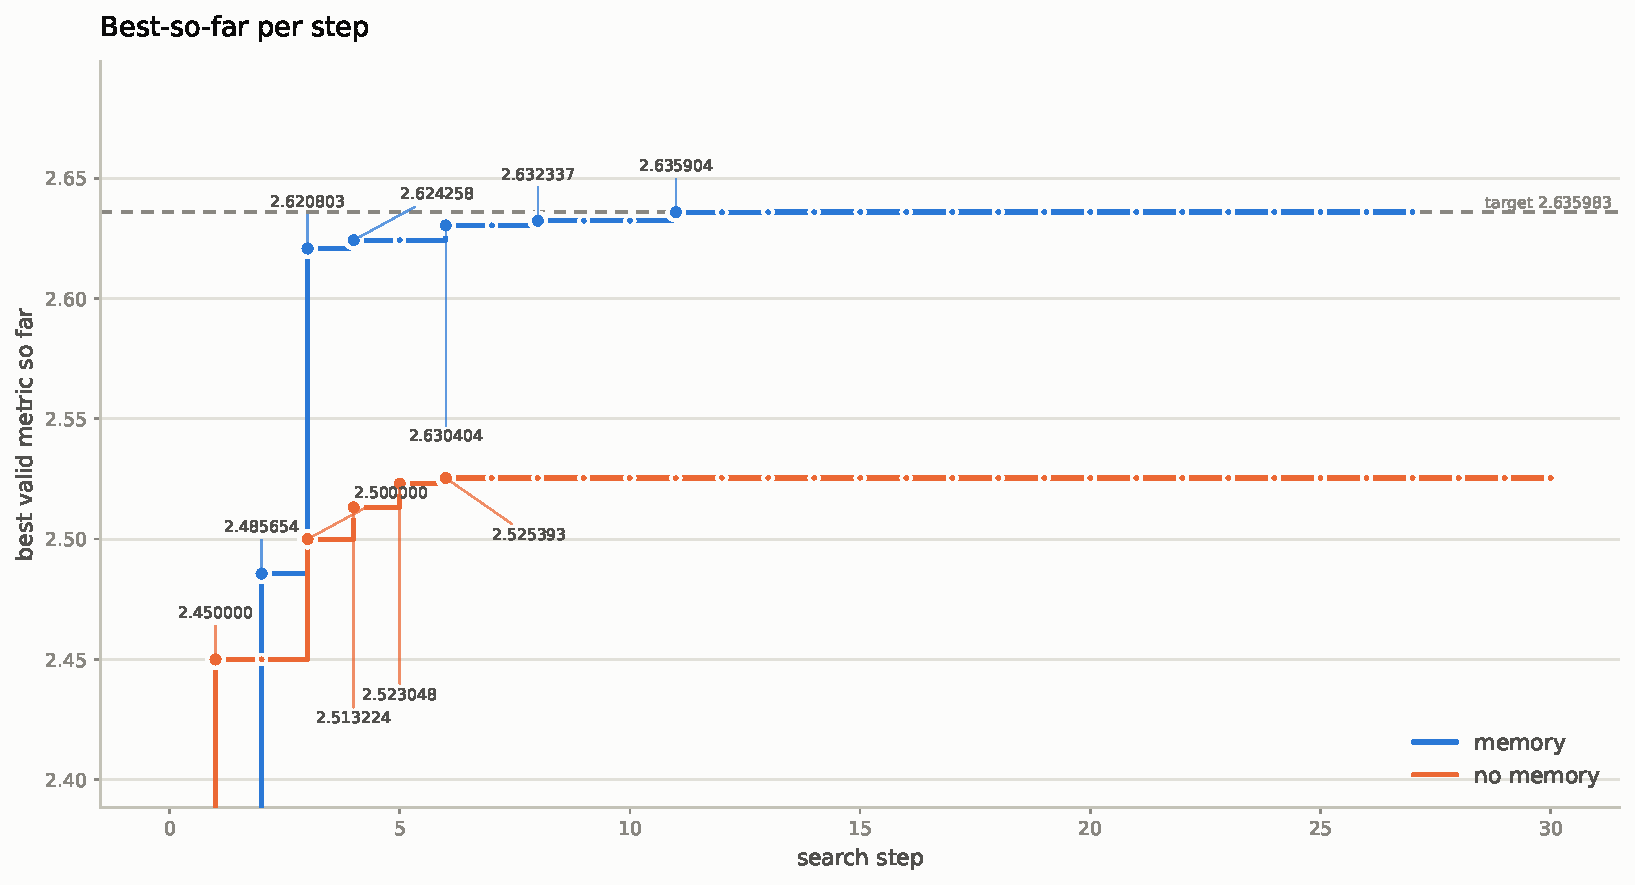
\includegraphics[width=\linewidth]{best_so_far.pdf}
\vspace{-1em}
\caption{Best score seen so far per training step. 
}
\label{fig:best}
\end{figure}
The two successful runs escaped by different routes, and a syntactic scan of the generated
programs (Table~\ref{tab:idioms}) identifies both. \textsc{mem-b} moved the radii into the
optimizer's decision vector, so that positions and radii are solved jointly; this appears in
$99.9\%$ of its programs after step $5$ and in about $1\%$ of the programs of the two runs
that never escaped. \textsc{mem-a} instead adopted global search (differential evolution,
basin hopping, or dual annealing) in $87.5\%$ of its late programs, against $28.7\%$ in
the control. The stalled run \textsc{mem-c} converged on the opposite pattern with a fixed
hexagonal seed followed by a greedy shrink, \texttt{radii[i] = min(radii[i], dist/2)}, in
$97.8\%$ of its programs. That construction caps the objective, because radii are never
enlarged once set.

\begin{table}[t]
\centering
\caption{Adoption of program idioms, as the fraction of generated responses at steps
$\geq 5$ matching a syntactic pattern. The last row matches the literal coordinate
expression stored in a single lesson of \textsc{mem-c}, reproduced in
Table~\ref{tab:lessons}.}
\label{tab:idioms}
\small
\begin{tabular}{lcccc}
\toprule
Idiom & \textsc{mem-a} & \textsc{mem-b} & \textsc{mem-c} & \textsc{no-mem} \\
\midrule
Global search (differential evolution / annealing) & \textbf{87.5} & 13.7 & 11.9 & 28.7 \\
Radii among the decision variables                 & 10.7 & \textbf{99.9} & 1.2 & 1.1 \\
Greedy shrink from a fixed seed                    & 71.9 & 7.4 & \textbf{97.8} & 25.6 \\
Verbatim grid formula from lesson \texttt{979e6dc0} & 0.7 & 0.0 & \textbf{99.0} & 0.0 \\
\bottomrule
\end{tabular}
\end{table}

\subsection{What the Memory Actually Contained and Used}

Retrieval collapsed onto a small fixed subset of memory. Across the three runs, $87\%$--$89\%$ of lessons were never retrieved, while the top five accounted for $60.1\%$--$76.8\%$ of all retrievals. Eq.~\ref{eq:memory-retrieval} explains this concentration. The task description and parent program change little across steps, so cosine similarity varies far less than the importance tilt $w=0.15$. Importance also provides little separation because $77\%$--$93\%$ of lessons receive the maximum score of $5$. Retrieval therefore repeatedly selects nearly the same entries.

These entries were not the lessons associated with successful search. All $48$ lessons describing global search, ensembles, or restarts received zero retrievals. Even \textsc{mem-b}'s escaping rollout was conditioned only on lessons describing the plateau it was leaving. The search behavior responsible for escape therefore entered through policy learning rather than retrieval.
% The bias is structural. 
Because the query is program text and similarity is lexical, code-like lessons match much more strongly than prose. Code forms only $23\%$--$34\%$ of each bank but receives $88.3\%$--$96.1\%$ of retrieval mass. The retriever thus favors the least transferable content.

The effect of this bias depends on what the retrieved code controls. The dominant lessons in \textsc{mem-a} and \textsc{mem-b} encode local repairs that compose with many global layouts. In contrast, \textsc{mem-c}'s \texttt{979e6dc0} directly fixes circle centers and therefore constrains the global solution structure. Its distinctive expression appears in $99.0\%$ of programs after step $5$, compared with $0.0\%$ in the control. For $n=26$, it also produces coincident centers, after which shrink-to-contact drives radii toward zero. A prose lesson expressing the same hexagonal idea in \textsc{mem-a} was never retrieved and caused no comparable lock-in. The relevant distinction is therefore not code versus prose alone, but whether a copied lesson constrains a local operation or instantiates the global construction.

\begin{table}[t]
\centering
\caption{The most-injected lesson of each run, and one that were never injected.
}
\label{tab:lessons}
\small
\setlength{\tabcolsep}{4pt}
\begin{tabular}{p{0.085\linewidth}p{0.04\linewidth}p{0.125\linewidth}p{0.55\linewidth}}
\toprule
ID & Run & Injected & Lesson text \\
\midrule
\texttt{979e6dc0} & \textsc{c} & 14{,}336 (19.3\%) &
{\ttfamily\scriptsize rows = int(np.ceil(np.sqrt(n)));\newline
cols = int(np.ceil(n / rows)); \dots\newline
x = 0.5 + (col - (cols-1)/2) * (1/(cols-1));\newline
y = 0.5 + (row - (rows-1)/2) * (1/(rows-1));\newline
if row \% 2 == 1: y += np.sqrt(3)/2 / 2} \\
\addlinespace
\texttt{1644ca11} & \textsc{b} & 17{,}600 (19.1\%) &
{\ttfamily\scriptsize for i in range(n): for j in range(i+1, n):\newline
dist = np.linalg.norm(centers[i] - centers[j]);\newline
radii[i] = min(radii[i], dist / 2);\newline
radii[j] = min(radii[j], dist / 2)} \\
\addlinespace
\texttt{d3b941ec} & \textsc{a} & 13{,}888 (15.5\%) &
Clamp circle positions to the unit square bounds during optimization:
{\ttfamily\scriptsize x = max(min(x, 1), 0), y = max(min(y, 1), 0)}. \\
\addlinespace
\texttt{3a29df87} & \textsc{a} & 0 (0.0\%) &
Initialize centers with a hexagonal grid layout for $n$ circles, adjusting spacing to fit the unit square. \\
\addlinespace
\bottomrule
\end{tabular}
\end{table}

Two properties of extraction further limit learning. First, positives are the $k$ highest-reward responses, so they become indistinguishable on plateaus. The median reward spread is $0.000000$ for \textsc{mem-b} and \textsc{mem-c}, with zero spread in $14/37$ and $16/30$ steps. The extractor therefore restates the current construction rather than identifying an improvement, since it never compares a child with its parent. Second, the deduplication threshold is ineffective. The $99$th percentile of lesson similarity is $0.647$, far below the $0.95$ threshold, so paraphrases enter as distinct lessons and further dilute the bank.
Acceptance rate is also a poor proxy for run quality. \textsc{mem-c} has the highest acceptance rate, $0.745$, but the lowest mean score because $13.46\%$ of accepted rollouts score zero, compared with $5.02\%$ and $3.33\%$ in the successful runs. Removing these zero-score rollouts eliminates most of its apparent advantage in valid$^{+}$ performance. Likewise, the run with no overlap violations never escaped, whereas the only run to reach the target sustained a $5.4\%$ overlap-failure rate. Searching near tangency requires approaching the constraint boundary.

\subsection{Implications for Memory Design}

The main failure is that memory stores instantiated constructions rather than transferable principles. Code occupies only a quarter to a third of each bank but receives $88$--$96\%$ of retrieval mass, while general lessons, including all $48$ lessons describing the search behavior associated with escape, are rarely retrieved. A system asked for principles but rewarded for lexical similarity will therefore converge on specifics.

The effect depends on what the retrieved rule controls. A local rule such as \textsc{mem-b}'s pairwise radius repair can transfer across programs without fixing the global search space. A global rule such as \textsc{mem-c}'s coordinate formula effectively specifies the solution and, with $99.0\%$ adoption versus $0.0\%$ in the control, turned the highest-traffic memory slot into a plateau. Memory should therefore preserve operations while leaving constructions free, allowing code for local repairs but requiring abstract descriptions for rules that determine global structure.

The measurements also suggest two mechanical changes. Retrieval must discriminate among lessons rather than collapse a bank of roughly $180$ entries into a fixed cache of five, and extraction should compare children with parents so that useful changes remain identifiable even when absolute rewards have plateaued.

Finally, these experiments do not isolate the effect of memory on final score. Only two escapes occurred across four runs, and configuration-identical runs differed by $0.12$. Future evaluations should therefore emphasize discovery events per unit of compute and include within-step controls, since every rollout after step $0$ here received memory injection.





\section{Test-Time Reinforcement Learning}
\label{sec:test-time-rl}

We adapt the generator online using LoRA while keeping the backbone weights
fixed. At iteration step $t$, let $\bar{\theta}$ denote the policy parameters
used to generate the current rollouts. The sampled responses are grouped by
their generating prompt as group $g_p$ contains the $G_p$ responses
$\{y_i\}_{i\in g_p}$ generated from the same prompt $x_p$. Each response
receives a scalar reward $r_i$ and, when unsuccessful, textual feedback $f_i$.
The update uses two complementary learning signals. The reward signal compares
responses generated from the same prompt, while the feedback signal provides
token-level information about failed responses.

\paragraph{Group-relative reward signal.}
Within each group $g_p$, we exponentially tilt the rewards using parameter $\beta\geq 0$ that controls how strongly the update favors the best responses. So we got:
\begin{equation}
\omega_i
=
\frac{
G_p \exp(\beta r_i)
}{
\displaystyle\sum_{j\in g_p}\exp(\beta r_j)
},
\qquad
A_i^{\mathrm{rew}}
=
\omega_i-1,
\qquad i\in g_p,
\label{eq:reward-advantage}
\end{equation}
As $\beta\rightarrow\infty$, the weight concentrates
on the highest-reward response. When the maximum is unique, its advantage
approaches $G_p-1$, while the remaining advantages approach $-1$. Hence,
$\beta$ smoothly controls the transition from mean-seeking to max-seeking
optimization.

\paragraph{Feedback-based failure signal.}
A scalar reward indicates whether a response succeeded, but it does not explain
which tokens contributed to its failure. We therefore reuse the rollout policy
as a feedback-conditioned self-teacher.
For a failed response $y_i$, define
\begin{equation*}
q_{\bar{\theta}}
\left(
v
\mid
x_p,f_i,y_{i,<\ell}
\right)
=
\pi_{\bar{\theta}}
\left(
v
\mid
\operatorname{reprompt}(x_p,f_i),y_{i,<\ell}
\right),
\label{eq:self-teacher}
\end{equation*}
where $\operatorname{reprompt}(x_p,f_i)$ augments the original prompt with the
evaluator feedback, $y_{i,<\ell}$ is the response prefix, and $v$ denotes a
candidate next token. The teacher and rollout policy use the same model
parameters; they differ only in whether the feedback is included in the
context.
For the sampled token $y_{i,\ell}$, the feedback-based advantage is
\begin{equation}
A_{i,\ell}^{\mathrm{fb}}
=
\log
q_{\bar{\theta}}
\left(
y_{i,\ell}
\mid
x_p,f_i,y_{i,<\ell}
\right)
-
\log
\pi_{\bar{\theta}}
\left(
y_{i,\ell}
\mid
x_p,y_{i,<\ell}
\right).
\label{eq:feedback-advantage}
\end{equation}
This quantity is computed once and detached from the optimization graph.
It is positive when the feedback makes the sampled token more plausible and
negative when the feedback-conditioned teacher considers that token less
appropriate. The textual feedback is therefore converted into dense,
token-level credit without training a separate reward model.


\paragraph{Online policy update.}
Define the failure indicator
$d_i
=
\mathbf{1}
\left\{
r_i=0
\ \text{or the attempt failed}
\right\},$
The group-relative reward signal and the feedback signal are combined into one
per-token advantage:
\begin{equation*}
A_{i,\ell}
=
A_i^{\mathrm{rew}}
+
\lambda_f d_i A_{i,\ell}^{\mathrm{fb}},
\qquad
\lambda_f\geq 0.
\label{eq:combined-advantage}
\end{equation*}
Successful responses are updated using only their group-relative reward.
Failed responses also receive the dense feedback term, which identifies which
parts of the response should be reinforced or discouraged. The coefficient
$\lambda_f$ controls the influence of this token-level correction.
Let $\theta$ denote the updated policy parameters and let
$\bar{\theta}$ denote the frozen rollout policy. The per-token importance ratio
is
\begin{equation}
\rho_{i,\ell}(\theta)
=
\frac{
\pi_{\theta}
\left(
y_{i,\ell}\mid x_p,y_{i,<\ell}
\right)
}{
\pi_{\bar{\theta}}
\left(
y_{i,\ell}\mid x_p,y_{i,<\ell}
\right)
}.
\label{eq:importance-ratio}
\end{equation}
The LoRA parameters are optimized using the objective
\begin{align}
\mathcal{L}(\theta)
=
-
\frac{1}{N_t}
\sum_p
\sum_{i\in g_p}
\sum_{\ell=1}^{|y_i|}
\min
\Bigl(
\rho_{i,\ell}(\theta)A_{i,\ell},
\nonumber
% &\hspace{45mm}
\operatorname{clip}
\bigl( &
\rho_{i,\ell}(\theta), 
1-\epsilon,
1+\epsilon
\bigr)
A_{i,\ell}
\Bigr)
\nonumber\\
&+
\eta_{\mathrm{KL}}\,
\mathbb{E}_{c\sim\mathcal{C}_t}
\left[
D_{\mathrm{KL}}
\left(
\pi_{\theta}(\cdot\mid c)
\,\Vert\,
\pi_{\theta_0}(\cdot\mid c)
\right)
\right],
\label{eq:test-time-rl-loss}
\end{align}
where
$N_t
=
\sum_p\sum_{i\in g_p}|y_i|$
is the total number of sampled tokens, $\epsilon$ is the clipping threshold,
$\theta_0$ denotes the initial policy before test-time adaptation, and
$\eta_{\mathrm{KL}}$ controls the regularization toward that initial policy.
The contexts in $\mathcal{C}_t$ are taken from the current rollout batch.
One gradient update is performed after each evolution step. Only the LoRA
parameters are modified, making the adaptation inexpensive while allowing both
successful and failed rollouts to contribute useful training signal.





\section{Full Algorithm}

\begin{algorithm}[h]
\caption{\method: memory-augmented \dpuct{} search with failure-aware max-seeking test-time RL}
\label{alg:main}
\begin{algorithmic}[1]
\Require problem $d$; backbone $\pi_{\theta_0}$ with LoRA adapter; $n, k, m, L$; $\alpha, \lambda, \tau, c$; $\beta, \lambda_f$; steps $T_{\max}$
\State $(R, T) \gets \mathrm{get\_env}(d)$;\quad tree and $\Dset \gets \{\text{root}\}$;\quad $\Mem \gets \emptyset$
\State \Return $\arg\max_{s \in \Dset} R(s)$
\end{algorithmic}
\end{algorithm}





\newpage

\subsubsection*{Acknowledgments}


\bibliography{ref}
\bibliographystyle{iclr2026_conference}

\appendix



\end{document}


